\documentclass[tikz,border=4pt]{standalone}
\usepackage{ctex}
\usepackage{amsmath}
\usetikzlibrary{calc, arrows.meta}

\begin{document}
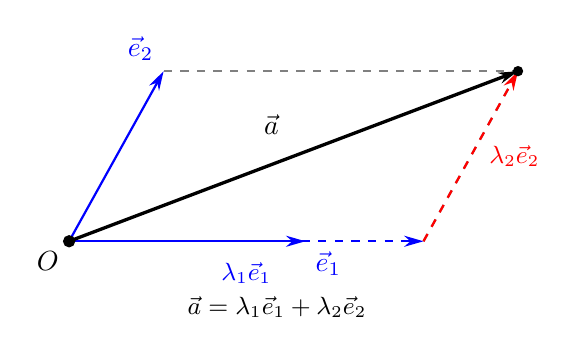
\begin{tikzpicture}[
  scale=1.2, thick,
  vec/.style={-{Stealth[length=7pt, width=4pt]}, thick},
]

% 基底 e1, e2（不共线的斜坐标系）
% e1 方向：水平向右
% e2 方向：斜上方（60°）
\coordinate (O) at (0, 0);
\coordinate (E1) at (2.5, 0);     % e1 端点
\coordinate (E2) at (1.0, 1.8);   % e2 端点

% 设 a = 1.5 e1 + 1 e2，所以 a 的端点是 E1*1.5/2.5 + E2
% 实际坐标：lambda1=1.5, lambda2=1.0
% P = O + 1.5*(2.5,0) + 1.0*(1.0,1.8) = (3.75+1.0, 0+1.8) = (4.75, 1.8)
\coordinate (A) at (4.75, 1.8);

% lambda1 * e1 的端点
\coordinate (P1) at (3.75, 0);  % O + 1.5*e1
% lambda2 * e2 的端点（从 P1 出发）
\coordinate (P2) at (4.75, 1.8); % P1 + 1.0*e2，即 = A

% 平行四边形辅助线（虚线）
\draw[dashed, gray] (P1) -- (A);          % 从 lambda1*e1 端点作平行于 e2 的线
\draw[dashed, gray] (E2) -- ++(3.75,0);   % 从 e2 端点作平行于 e1 方向延长线，
                                            % 到 (1+3.75, 1.8)=(4.75,1.8)=A  ✓

% 基底向量 e1, e2
\draw[vec, blue]  (O) -- (E1) node[below right] {$\vec{e}_1$};
\draw[vec, blue]  (O) -- (E2) node[above left]  {$\vec{e}_2$};

% 分量向量 lambda1*e1（蓝虚）
\draw[vec, blue, dashed] (O) -- (P1)
  node[below, midway, yshift=-4pt] {\small $\lambda_1\vec{e}_1$};

% 分量向量 lambda2*e2（从 P1 出发，红虚）
\draw[vec, red, dashed] (P1) -- (A)
  node[right, midway, xshift=3pt] {\small $\lambda_2\vec{e}_2$};

% 合向量 a
\draw[vec, black, very thick] (O) -- (A)
  node[above, midway, xshift=-8pt, yshift=4pt] {$\vec{a}$};

% 原点
\filldraw[black] (O) circle (1.5pt) node[below left] {$O$};
\filldraw[black] (A) circle (1.2pt);

% 等式说明
\node[font=\small] at (2.2, -0.7)
  {$\vec{a} = \lambda_1\vec{e}_1 + \lambda_2\vec{e}_2$};

\end{tikzpicture}
\end{document}
